\chapter{Polynomial Interpolation} \label{ch:polynomial}

Imagine we were given a set of $n+1$ data points $\{ (x_0,y_0)$, $(x_1,y_1)$, $\dots$, $(x_n,y_n) \}$ as shown in figure~\ref{fig:ch3_scatter}.
\begin{figure}[H]
	\begin{center}
	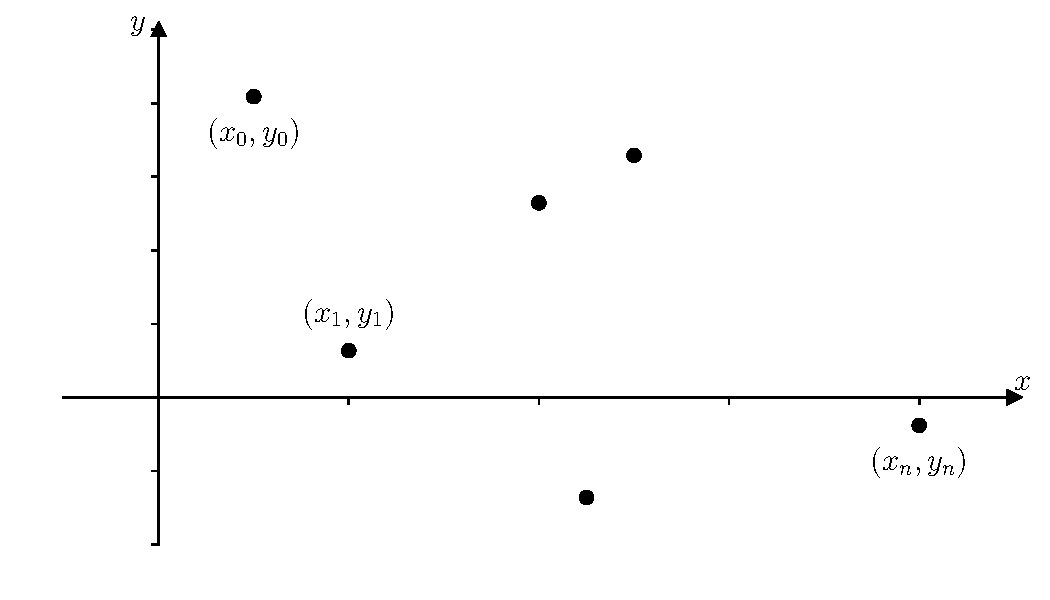
\includegraphics[width=0.7\textwidth]{figures/ch3_scatter.pdf} 
	  \caption{Scatter of $n+1$ points that we wish to fit.} \label{fig:ch3_scatter}
	\end{center}
\end{figure}
We may want to estimate what happens between the points. In this case it will be useful to have a function that agrees with the given data, but is defined for \textit{any} $x$ whatsoever. In this chapter we will consider polynomials to fill this role. Recall the definition of a polynomial of degree $n$
\begin{align*}
p(x) = a_0 + a_1 x + a_2 x^2 + \cdots + a_n x_n^n = \sum_{k=0}^n a_k x^k.
\end{align*}

As another motivation, we may be given a function $f(x)$ instead of data points. It can be computationally useful to estimate this function as a polynomial. Why? Maybe the function doesn't have a closed form. Maybe it takes a lot of computational power to give $f(x)$ at any particular $x$. In such a case you can compute a finite set of points $\{ (x_0,f(x_0))$, $(x_1,f(x_1))$, $\dots$, $(x_n,f(x_n)) \}$ that we can then use a polynomial to fit. The polynomial could then be used at a much reduced computational expense. On top of that, polynomials are analytically differentiable, which can be useful.


\section{Piece-wise linear fit}
We start with the simplest function that agrees with a set of data points: the \textit{piece-wise linear} fit that simply connects all the data points by straight lines, as sketched in figure~\ref{fig:ch3_piecewise}.
\begin{figure}[H]
	\begin{center}
	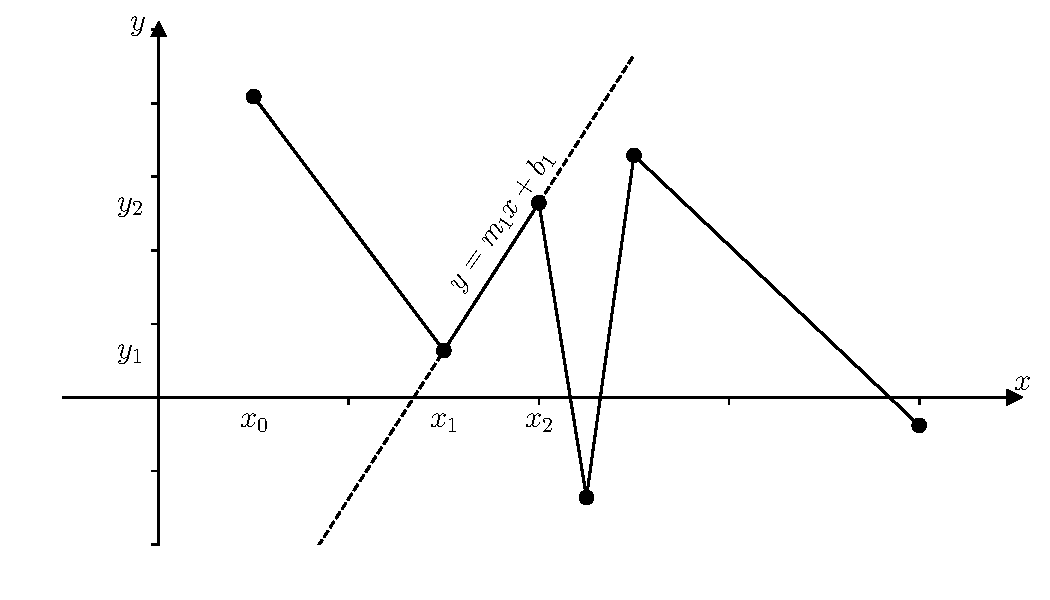
\includegraphics[width=0.8\textwidth]{figures/ch3_piecewise.pdf} 
	  \caption{Sketch of a piece-wise linear fit to some data points. The straight line connecting the 2nd and 3rd data points is highlighted.} \label{fig:ch3_piecewise}
	\end{center}
\end{figure}
It's necessary to order the data points in increasing $x$ coordinate, or else the resulting fit will be multi-valued, and thus not well defined. Then, for each pair of adjacent data points $(x_k,y_k)$ and $(x_{k+1},y_{k+1})$ we must define a straight line equation $y = m_k x + b_k$ for the interval between these points $x\in [x_k,x_{k+1}]$. The slope is given by ``rise over run'' for these two points
\begin{align*}
\boxed{ m_k = \frac{ y_{k+1}-y_{k} }{ x_{k+1}-x_{k} } }
\end{align*}
and then we get the $y$-intercept by using the straight line equation at either of the two data points
\begin{align*}
y(x_k) = y_k = m_k x_k + b_k \\
\implies \boxed{ b_k = y_k - m_k x_k} \\
(\text{or } b_k = y_{k+1} - m_k x_{k+1}).
\end{align*}
As defined above we have a function \textit{between} the data points. In principle we can just extend the first straight line infinitely to the left, $(-\infty,x_0]$, and also the last straight line infinitely to the right, $[x_n,\infty)$, in order to have a function defined for all $x\in \mathbb{R}$. Usually this is not a good idea.

\exemple{\upline}
{
	Find the piece-wise linear fit to the data: $\{ (1,1)$, $(2,3)$, $(3,2)$, $(4,3) \}$.
	
	For data points $(1,1)$, $(2,3)$:
	\begin{align*}
	& m_1 = \frac{3-1}{2-1} = 2 \\
	& b_1 = 1 - 2\times 1 = -1 \\
	& \implies y = 2x - 1
	\end{align*}
	
	For data points $(2,3)$, $(3,2)$:
	\begin{align*}
	& m_1 = \frac{2-3}{3-2} = -1 \\
	& b_1 = 3 - -1 \times 2 = 5 \\
	& \implies y = -x + 5
	\end{align*}
	
	For data points $(3,2)$, $(4,3)$:
	\begin{align*}
	& m_1 = \frac{3-2}{4-3} = 1 \\
	& b_1 = 2 - 1\times 3 = -1 \\
	& \implies y = x - 1
	\end{align*}
	
	So we can define the function on any $x$ between the first and last data point
	\begin{align*}
	y(x) = 
	\begin{cases}
	2x - 1 & \text{for } x\in [1,2] \\
	-x + 5 & \text{for } x\in [2,3] \\
	 x - 1 & \text{for } x\in [3,4] 
	\end{cases}
	\end{align*}
}{\downline}


\section{Lagrangian interpolation}
In this method, we fit a smooth polynomial through the scattering of points. Recall the figure~\ref{fig:ch3_scatter}, where we have $n+1$ pairs of numbers $(x_k,y_k)$. Let's start with a theorem

\theorem{LAGRANGE INTERPOLATION }{}
{Given the $n+1$ unique points $(x_0,y_0)$, $(x_1,y_1)$, $\dots$, $(x_n,y_n)$, there is a unique polynomial of degree at most $n$ passing through each point. That is, 
\begin{gather*}
\exists p_n(x) \in \mathcal{P}_n \\
\text{such that}\\ 
p_n(x_k)=y_k \quad \forall k.
\end{gather*}
}

We'll spend the rest of this section constructing this unique polynomial, called the \textit{Lagrange polynomial}.

First let's consider a couple of trivial cases. If we have just 1 point, $(x_0,y_0)$, then the degree 0 polynomial
\begin{align*}
p_0(x) = y_0
\end{align*}
will pass through the point. Though there are infinite straight lines that could go through this single point, this horizontal line is the only \textit{degree 0 polynomial}. When we have 2 points $(x_0,y_0)$ and $(x_1,y_1)$ then the degree 1 polynomial Lagrange polynomial is just the straight line joining the two
\begin{align*}
& p_1(x) = mx + b \\
& \text{with} \quad m = \frac{y_1 - y_0}{x_1 - x_0} \quad \text{and} \quad  b = m x_0 - y_0.
\end{align*}
These two trivial cases are shown in figure~\ref{fig:ch3_lagrange_n0_n1}.
\begin{figure}[H]
	\begin{center}
	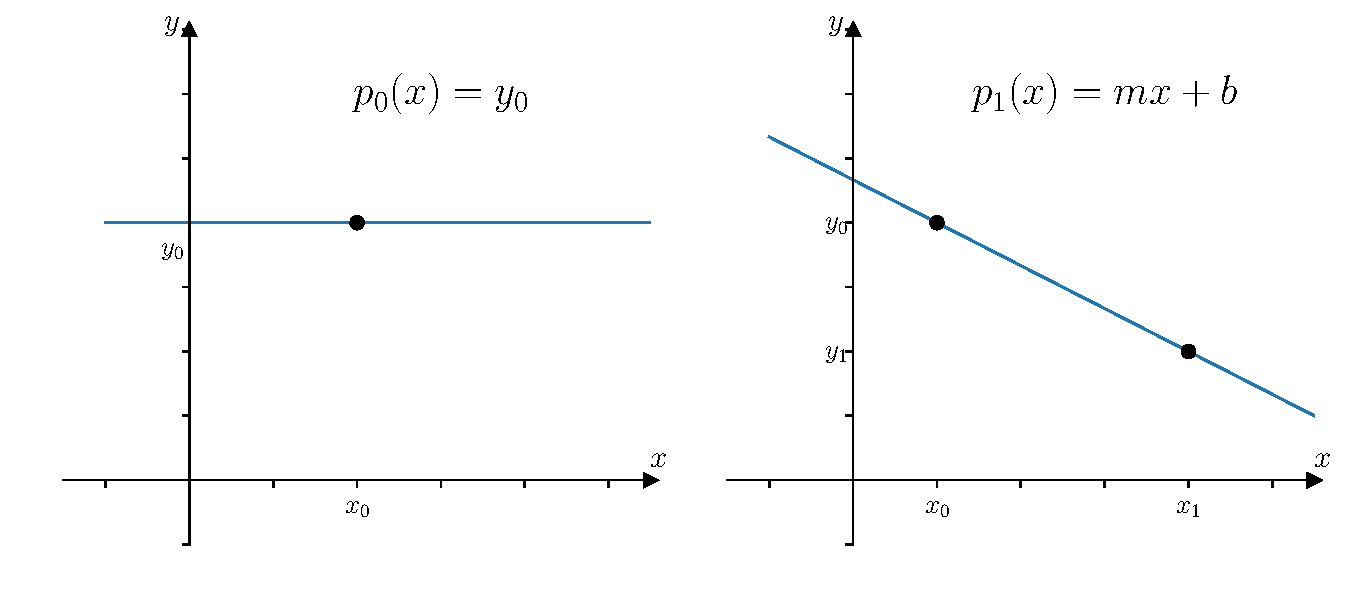
\includegraphics[width=\textwidth]{figures/ch3_lagrange_n0_n1.pdf} 
	  \caption{Trivial Lagrange polynomials for $n=0$ and $n=1$.} \label{fig:ch3_lagrange_n0_n1}
	\end{center}
\end{figure}

Ok, let's construct this unique polynomial for when we have more than 2 points. First, we choose one of the points, so $(x_k, y_k)$, and construct a polynomial, call it $L_k(x)$, that passes through 1 at this $x$, and goes through zero at all the other positions $x_i$ for $i\neq k$. That is, $L_k(x)$ must pass through the points $(x_k,1)$ and $(x_i,0)$ for all $i\neq k$. This polynomial is sketched in figure~\ref{fig:ch3_lagrange_Lk}.
\begin{figure}[H]
	\begin{center}
	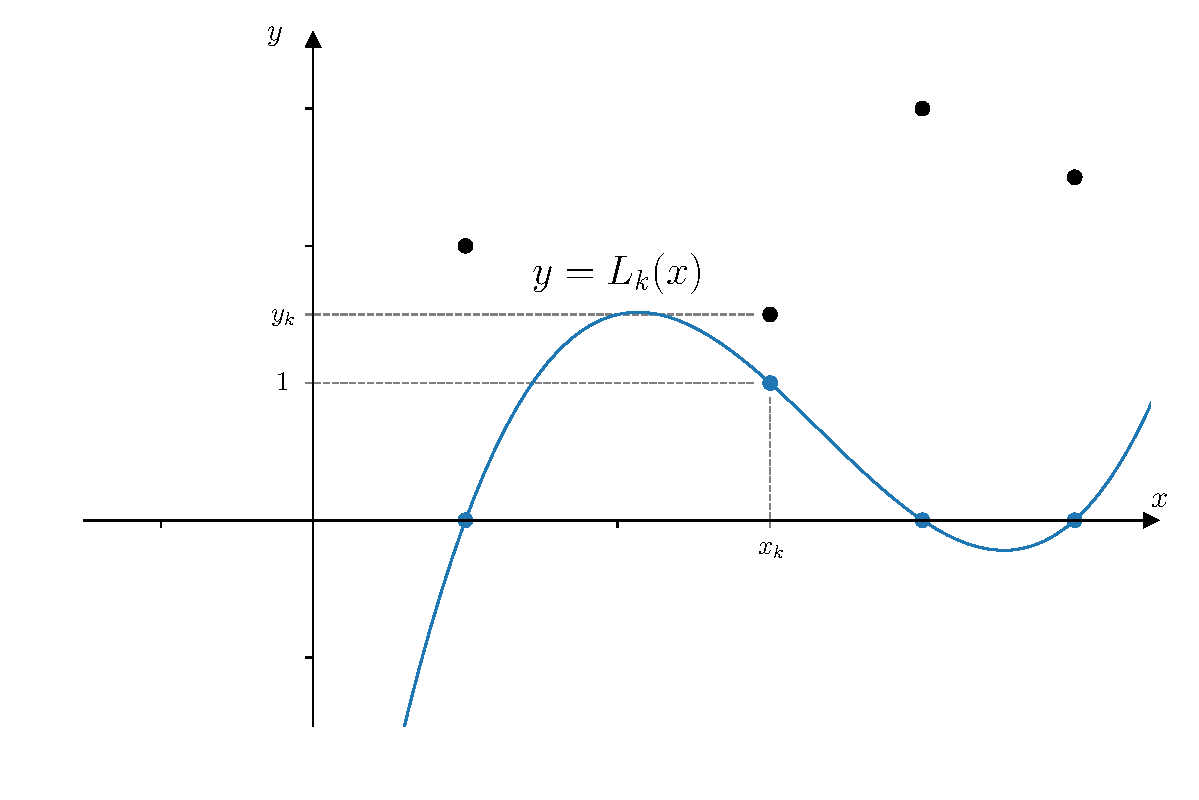
\includegraphics[width=0.6\textwidth]{figures/ch3_lagrange_Lk.pdf} 
	  \caption{.} \label{fig:ch3_lagrange_Lk}
	\end{center}
\end{figure}

It's very simple to construct a polynomial that has zeros at chosen $x$ values:
\begin{align*}
L_k(x) \propto (x-x_0)(x-x_1)\times \dots \times(x-x_{k-1})(x-x_{k+1})\times \dots \times(x-x_{n}).
\end{align*}
Notice we have excluded a term like $(x-x_k)$ to ensure that $L_k(x)$ \textit{does not} equal 0 at $x=x_k$. Including the proportionality constant, we then have
\begin{align*}
L_k(x) = C_k \prod_{i\neq k} (x-x_i).
\end{align*}
If you're not familiar with the ``big pie'' notation, it is the multiplicative version of the ``big sigma'' summation symbol $\Sigma$. Formally it is
\begin{align*}
\prod_{i=j}^{N} a_i = a_j \times a_{j+1} \times a_{j+2} \times \cdots \times a_{N-1} \times a_{N}.
\end{align*}
It just means that we multiply the following expression by itself over the indices provided. Look at the previous expression for $L_k(x)$ to see what the $\prod$ symbol is replacing.

Now, we can determine the constant $C_k$ by following our other desired property of $L_k(x)$, that it passes through $(x_k,1)$. This means
\begin{align*}
& L_k(x_k) = 1 \\
& \implies C_k \prod_{i\neq k} (x_k-x_i) = 1 \\
& \implies C_k  = \frac{1}{\prod_{i\neq k} (x_k-x_i)}
\end{align*}
So now we can write the definition of $L_k(x)$ in terms of the coordinates we are trying to fit
\begin{align*}
L_k(x) = \frac{\prod_{i\neq k} (x-x_i)}{\prod_{i\neq k} (x_k-x_i)}  = \prod_{i\neq k} \frac{x-x_i}{x_k-x_i} 
\end{align*}
Look at this function carefully. The denominator will be a multiplication of differences of known numbers, and so it will result in some number. The numerator is a function of $x$. We'll see in examples how this works in practice, but it really is just a number multipled by a polynomial, cleverly constructed to pass through certain points.

Now, this function passes through $(x_k,1)$ and $(x_i,0)$ for all $i\neq k$. If we multiply $L_k(x)$ by $y_k$, we will have a new polynomial that passes through $(x_k,y_k)$ and doesn't change the other points that still must pass through zero. This, therefore, nicely gives us the properties we wanted from the beginning 
\begin{align*}
y_k L_k(x) = 
\begin{cases}
y_k & \quad \text{if } x=x_k \\
0 & \quad \text{if } x=x_i \text{ for } i\neq k. 
\end{cases}
\end{align*} 
Now we only have to add up a series of these polynomials, giving us a new polynomial, that passes through every point we want. This is the \textit{Lagrange polynomial}:
\begin{align*}
\boxed{p(x) = \sum_{k=0}^n y_k L_k(x)}
\end{align*}
The components of the polynomial, $L_k(x)$, are called \textit{Lagrange basis polynomials}. A sketch of a Lagrange polynomial and its basis polynomials is shown in figure~\ref{fig:ch3_lagrange_total}.
\begin{figure}[H]
	\begin{center}
	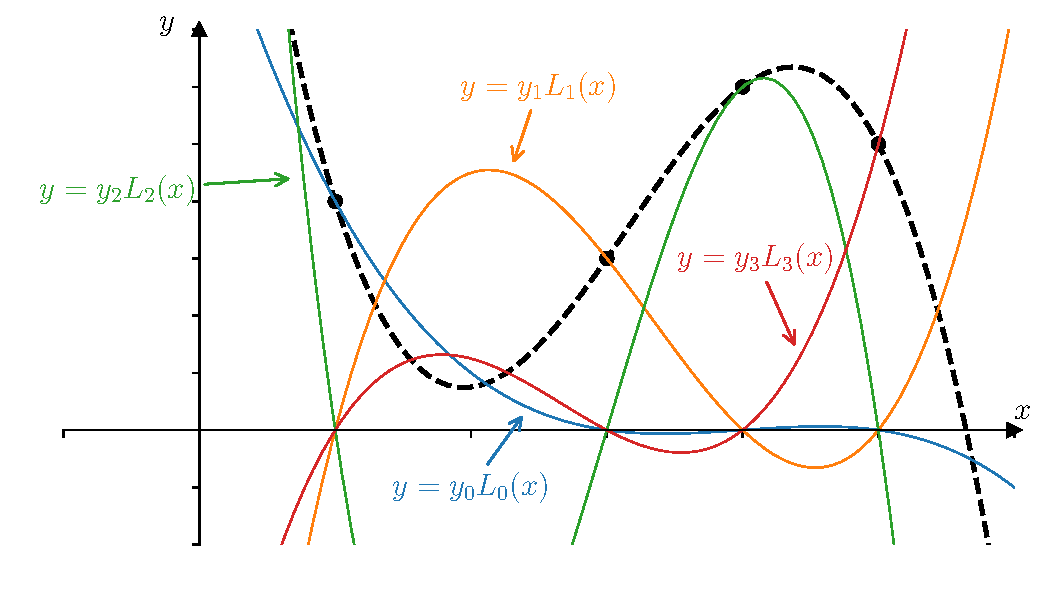
\includegraphics[width=0.8\textwidth]{figures/ch3_lagrange_total.pdf} 
	  \caption{Terms of the Lagrange polynomial. Note that each coloured line passes through exactly 1 of the desired interpolation points, while passing through zero at the location of all the others. The dashed line is the addition of the other 4 lines, and thus passes through each interpolation point.} \label{fig:ch3_lagrange_total}
	\end{center}
\end{figure}

\exemple{\upline}
{
	Let's find the Lagrange polynomial that passes through the points in 
	\begin{align*}
	\{(x_0,y_0),(x_1,y_1),(x_2,y_2),(x_3,y_3)\}=\{(1,1),(2,3),(3,2),(4,3)\}.
	\end{align*}
	Since there are 4 points to fit, we form 4 basis polynomials
	\begin{align*}
	L_0(x) &= \frac{(x-2)(x-3)(x-4)}{(1-2)(1-3)(1-4)}  = -\frac{1}{6}(x-2)(x-3)(x-4) \\ \\
	L_1(x) &= \frac{(x-1)(x-3)(x-4)}{(2-1)(2-3)(2-4)}  =  \frac{1}{2}(x-1)(x-3)(x-4) \\ \\
	L_2(x) &= \frac{(x-1)(x-2)(x-4)}{(3-1)(3-2)(3-4)}  = -\frac{1}{2}(x-1)(x-2)(x-4) \\ \\
	L_3(x) &= \frac{(x-1)(x-2)(x-3)}{(4-1)(4-2)(4-3)}  =  \frac{1}{6}(x-1)(x-2)(x-3)
	\end{align*} 
	Stare at each polynomial until you recognise the patterns. In this first step, the denominator is a copy/paste of the numerator, but $x$ is replaced with $x_k$ where $k$ is the index of the basis polynomial you are considering. Finally, we must add up these basis polynomials multipled by the $y$ values of the fitting points
	\begin{align*}
	p(x) &= 1\times L_0(x) + 3\times L_1(x) + 2\times L_2(x) + 4\times L_3(x)  \\
	 &= -\frac{1}{6}(x-2)(x-3)(x-4) + \frac{3}{2}(x-1)(x-3)(x-4) \\
		& - (x-1)(x-2)(x-4) + \frac{2}{3}(x-1)(x-2)(x-3)
	\end{align*}
}{\downline}




\subsection{Interpolation error estimation}
We can use a Lagrange polynomial to approximate a function $f(x)$ by sampling it at $n+1$ points $x_0$, \dots, $x_n$. That is, we take as data points $(x_0,f(x_0))$, $(x_1,f(x_1))$, \dots, $(x_n,f(x_n))$. If the function is continuous on the interval of the interpolation $[x_0,x_n]$, and its derivative of order $n+1$ exists and is also continuous on that interval, then the interpolation error is bounded:
\begin{align*}
|f(x) - p_n(x)| \leq \frac{M_{n+1}}{(n+1)!} \left| \prod_{i=0}^n (x-x_i) \right|
\end{align*}
where 
\begin{align*}
M_{n+1} = \max_{\alpha \in [x_0,x_n]} \left| f^{(n+1)}(\alpha)\right|
\end{align*}

%%%%%%%%%%%%%%%%%%%%%%%%%%%%%%%%%%%%%%%%%%%%%%
%%%%%%%%%%%%%%%%%%%%%%%%%%%%%%%%%%%%%%%%%%%%%%
%%%%%%%%%%%%%%%%%%%%%%%%%%%%%%%%%%%%%%%%%%%%%%
%%%%%%%%%%%%%%%%%%%%%%%%%%%%%%%%%%%%%%%%%%%%%%






%%%%%%%%%%%%%%%%%%%%%%%%%%%%%%%%%%%%%%%%%%%%%%
%%%%%%%%%%%%%%%%%%%%%%%%%%%%%%%%%%%%%%%%%%%%%%
%%%%%%%%%% NEWTONIAN INTERPOLATION %%%%%%%%%%%
%%%%%%%%%%%%%%%%%%%%%%%%%%%%%%%%%%%%%%%%%%%%%%
%%%%%%%%%%%%%%%%%%%%%%%%%%%%%%%%%%%%%%%%%%%%%%
\section{Newtonian interpolation}
There is a weakness to the Lagrangian method for finding the interpolation polynomial. Consider a set of $n+1$ data points $(x_0,y_0), (x_1,y_1), \dots, (x_n,y_n)$, so that the Lagrange polynomial is
\begin{align*}
p_n(x) = \sum_{k=0}^n y_k \prod_{i\neq k} \frac{x-x_i}{x_k-x_i} 
\end{align*}
what happens if we add data point $(x_{n+1},y_{n+1})$, as pictured below?
\begin{figure}[H]
	\begin{center}
	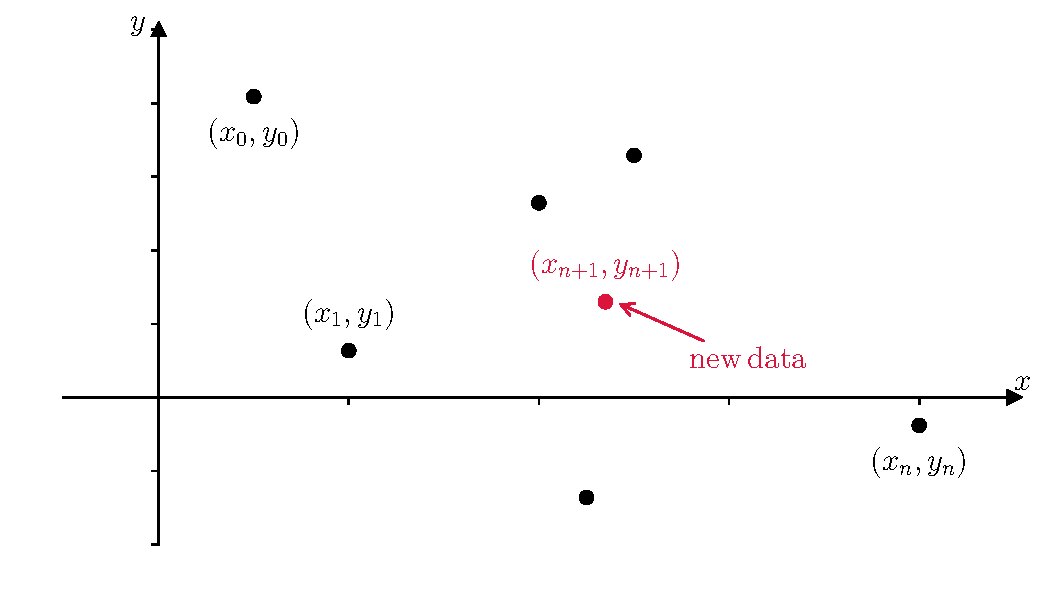
\includegraphics[width=0.8\textwidth]{figures/ch3_newton_purpose.pdf} 
	  \caption{} \label{fig:ch3_newton_purpose}
	\end{center}
\end{figure}

Well we would have to recompute all the Lagrange basis polynomials again to find $p_{n+1}$. This is obviously cumbersome, so we would like a method for \textit{sequentially} building the unique interpolation polynomial out of the previous polynomial with 1 less point and therefore 1 lower degree. That is, we want a scheme
\begin{align}\label{eq:ch3_newton_scheme}
p_{n+1}(x) = p_n(x) + q_{n+1}(x), \quad q_{n+1}(x) \in \mathcal{P}_{n+1}.
\end{align}
Now, the new polynomial must pass through all of the old points, so
\begin{align*}
p_{n+1}(x_k) = y_k \quad {\rm for} \, k=0,1,\dots,n.
\end{align*}
We also have that the old polynomial obviously passes through the old points
\begin{align*}
p_n(x_k) = y_k \quad {\rm for} \, k=0,1,\dots,n.
\end{align*}
Hence equation~\ref{eq:ch3_newton_scheme} evaluated at one of the data points gives
\begin{align*}
 p_{n+1}(x_k) &= p_n(x_k) + q_{n+1}(x_k) \\
 y_k &= y_k + q_{n+1}(x_k).
\end{align*}
So we have the constraint
\begin{align*}
q_{n+1}(x_k) = 0 \quad {\rm for} \, k=0,1,\dots,n.
\end{align*}
This means the general form of this extension polynomial is
\begin{align*}
q_{n+1}(x) = C_{n+1} \prod_{i=0}^{n} (x-x_i)
\end{align*}
for some constant $C_{n+1}$. Now the new polynomial, $p_{n+1}$ must also pass through the new datapoint $(x_{n+1},y_{n+1})$, giving
\begin{align*}
p_{n+1}(x_{n+1}) = y_{n+1}
\end{align*}
and hence
\begin{align*}
& y_{n+1} = p_n(x_{n+1}) + q_{n+1}(x_{n+1}) \\
&\implies C_{n+1} \prod_{i=0}^{n} (x_{n+1}-x_i) = y_{n+1} - p_n(x_{n+1}).
\end{align*}
This gives us an expression for this constant in terms of known values
\begin{align*}
\boxed{C_{n+1} = \frac{y_{n+1} - p_n(x_{n+1})}{\prod_{i=0}^{n} (x_{n+1}-x_i)}. }
\end{align*}
And so the Newtonian interpolation polynomial is given recursively as:
\begin{align}\label{eq:ch3_newton_scheme_explicit}
\boxed{p_{n+1}(x) = p_n(x) + C_{n+1}\prod_{i=0}^{n} (x-x_i).}
\end{align}
Let's look at this expression sequentially. The zeroth term is simple, it's forced to be a 0 degree polynomial passing through the point $(x_0,y_0)$. That is, it must be $p_0(x)=y_0$. This starts us off and let's us use equation~\ref{eq:ch3_newton_scheme_explicit}
\begin{align*}
p_1(x) &= y_0 + C_1(x-x_0) \\
%
p_2(x) &= y_0 + C_1(x-x_0) + C_2(x-x_0)(x-x_1) \\
%
&\vdots \\
%
p_{n+1}(x) &= y_0 + C_1(x-x_0) + C_2(x-x_0)(x-x_1) + \cdots +  C_{n+1}(x-x_0)(x-x_1)\times \dots \times (x-x_n)
\end{align*}

Now, $C_{n+1}$ as given above is horribly impractible. Let's demonstrate that by finding $C_1$ and $C_2$ in the general case before looking at a much better method!
\begin{align*}
C_1 &= \frac{y_1 - p_0(x_1)}{x_1-x_0} = \frac{y_1 - y_0}{x_1-x_0} \\
C_2 &= \frac{y_2 - p_1(x_2)}{(x_2-x_0)(x_2-x_1)} \\
%
&= \frac{y_2 - (y_0 + C_1(x_2-x_0))}{(x_2-x_0)(x_2-x_1)} \\
%
&= \frac{y_2 - y_0 - \frac{y_1 - y_0}{x_1-x_0}(x_2-x_0)}{(x_2-x_0)(x_2-x_1)} \\
%
&= \frac{y_2 - y_0}{(x_2-x_0)(x_2-x_1)} - \frac{y_1 - y_0}{(x_1-x_0)(x_2-x_1)}
%
\end{align*}
You see that the complexity builds up quickly. Try to write down $C_3$. But, there is a nice trick to quickly compute these coefficients, called \textit{divided differences}.

First, notationally we will replace the $C_{n+1}$ with
\begin{align*}
C_{n+1} = [y_0,\dots,y_n,y_{n+1}].
\end{align*}
This turns out to have a nice pattern involving recursive differences
\begin{align*}
C_0 &= [y_0] = y_0 \\
%
C_1 &= [y_0,y_1] = \frac{y_1 - y_0}{x_1-x_0} \\
%
C_2 &= [y_0,y_1,y_2] = \frac{[y_1,y_2] - [y_0,y_1]}{x_2-x_0} \\
%
C_3 &= [y_0,y_1,y_2,y_3] = \frac{[y_1,y_2,y_3] - [y_0,y_1,y_2]}{x_3-x_0} \\
%
&\vdots \\
%
C_{n+1} &= [y_0,\dots,y_n,y_{n+1}] = \frac{[y_1,\dots,y_{n+1}] - [y_0,\dots,y_{n}]}{x_{n+1}-x_0}.
\end{align*}
Before we make this clearer, let's check that it gives the right expression for $C_2$, that we found earlier.
\begin{align*}
C_2 &= \frac{[y_1,y_2] - [y_0,y_1]}{x_2-x_0} \\
%
&= \frac{\frac{y_2 - y_1}{x_2-x_1}  - \frac{y_1 - y_0}{x_1-x_0} }{x_2-x_0}  \\
%
&= \frac{y_2 - y_1}{(x_2-x_1)(x_2-x_0)} - \frac{y_1 - y_0 }{(x_1-x_0)(x_2-x_0)} \\
%
&= \frac{y_2 - y_0 + y_0 - y_1}{(x_2-x_1)(x_2-x_0)} - \frac{y_1 - y_0 }{(x_1-x_0)(x_2-x_0)}    \\
%
&= \frac{y_2 - y_0}{(x_2-x_1)(x_2-x_0)}- \frac{y_1 - y_0}{(x_2-x_1)(x_2-x_0)} - \frac{y_1 - y_0 }{(x_1-x_0)(x_2-x_0)} \\
%
&= \frac{y_2 - y_0}{(x_2-x_1)(x_2-x_0)}- \frac{y_1 - y_0}{x_2-x_0}\left(\frac{1}{x_2-x_1} +\frac{1}{x_1-x_0} \right) \\
%
&= \frac{y_2 - y_0}{(x_2-x_1)(x_2-x_0)}- \frac{y_1 - y_0}{(x_2-x_1)(x_1-x_0)}.
\end{align*}
It took some tricks but we got there, it's the same expression!

So, all we have done so far is replace one weird expression, the $C_{n+1}$, with another, $[y_0,\dots,y_n]$. If we compute these new things the interpolation polynomial is given by
\begin{align*}
p_{n+1}(x) &= [y_0] + [y_0,y_1](x-x_0) + [y_0,y_1,y_2](x-x_0)(x-x_1) + \cdots \\
& \quad + [y_0,\dots,y_{n+1}](x-x_0)(x-x_1)\times \cdots \times (x-x_n).
\end{align*}

Now we come to the heart of the method. These coefficients can be organised into a table that makes their computation actually clear:

\noindent \fbox{\begin{minipage}{\linewidth}
\underline{\textbf{Table of divided differences for Newtonian interpolation}}
\begin{figure}[H]
\begin{tabular}{ll|lll}
$x_0$ & $[y_0]$ &             &                 & \\ 
      &         & $[y_0,y_1]$ &                 & \\ 
$x_1$ & $[y_1]$ &             & $[y_0,y_1,y_2]$ & \\ 
      &         & $[y_1,y_2]$ &                 & $[y_0,y_1,y_2,y_3]$ \\ 
$x_2$ & $[y_2]$ &             & $[y_1,y_2,y_3]$ & \\ 
      &         & $[y_2,y_3]$ &                 & \\ 
$x_3$ & $[y_3]$ &             &                 & \\
\vdots & \vdots & \vdots & \vdots & \vdots
\end{tabular}
\end{figure}

\end{minipage}}

And of course it will become clearer what this table means with multiple usages.

\exemple{\upline}{
Given the data $\{(1,2), (2,2), (3,1), (4,3) \}$, determine the interpolation polynomial using the table of divided differences.

The table of divided differences is
\begin{figure}[H]
\begin{tabular}{ll|lll}
$x_k$ & $y_k$ &  &  & \\ \hline
$1$ & \fbox{2} &                      &                                 & \\ 
    &   & $\frac{2-2}{2-1}=\fbox{0}$  &                                 & \\ 
$2$ & 2 &                      & $\frac{-1-0}{3-1}=\fbox{-1/2}$ & \\ 
    &   & $\frac{1-2}{3-2}=-1$ &                                 &  $\frac{\frac{3}{2}--\frac{1}{2}}{4-1}=\fbox{2/3}$ \\ 
$3$ & 1 &                      & $\frac{2--1}{4-2}=\frac{3}{2}$  & \\ 
    &   & $\frac{3-1}{4-3}=2$  &                                 & \\ 
$4$ & 3 &                      &                                 &
\end{tabular}
\end{figure}
In the boxes are the coefficients we need for the interpolation polynomial
\begin{align*}
p(x) &= 2 + 0(x-1) - \frac{1}{2}(x-1)(x-2) + \frac{2}{3}(x-1)(x-2)(x-3) \\
&= 2 - \frac{1}{2}x^2 + \frac{3}{2}x - 1 +\frac{2}{3}x^3 - 4 x^2 + \frac{22}{3}x - 4 \\
&= -3 + \frac{53}{6}x - \frac{9}{2}x^2 + \frac{2}{3}x^3
\end{align*}
}{\downline}

Now let's do an example to see that \textit{the order of the data doesn't matter}.

\exemple{\upline}{
Given the data $\{(1,2), (3,1), (4,3) \}$, construct the table of divided differences. Then add the datapoint $(2,2)$ to find the interpolation polynomial.

The table of divided differences for the 3 points is
\begin{figure}[H]
\begin{tabular}{ll|lll}
$x_k$ & $y_k$ &  &  & \\ \hline
$1$ & $\fbox{2}$ &                               & & \\ 
    &            & $\frac{1-2}{3-1}=\fbox{-1/2}$ & & \\ 
$3$ & $1$        &                               & $\frac{2--\frac{1}{2}}{4-1}=\fbox{5/6}$  & \\ 
    &            & $\frac{3-1}{4-3}=2$           & &  \\ 
$4$ & $3$        &                               & & \\ 
\end{tabular}
\end{figure}
In the boxes are the coefficients we need for the degree 2 polynomial fitting just these 3 points
\begin{align*}
p_2(x) &= 2 - \frac{1}{2}(x-1) + \frac{5}{6}(x-1)(x-3) \\
&= 2 - \frac{1}{2}x + \frac{1}{2} +\frac{5}{6}x^2 -\frac{10}{3}x + \frac{5}{2}\\
&= 5 - \frac{23}{6}x + \frac{5}{6}x^2
\end{align*}
Now we add the new point $(2,2)$ by simply attaching it to the previous table
\begin{figure}[H]
\begin{tabular}{ll|lll}
$x_k$ & $y_k$ &  &  & \\ \hline
$1$ & $2$ &                               & & \\ 
    &     & $\frac{1-2}{3-1}=-\frac{1}{2}$ & & \\ 
$3$ & $1$ &                               & $\frac{2--\frac{1}{2}}{4-1}=\frac{5}{6}$ & \\ 
    &     & $\frac{3-1}{4-3}=2$           &                                          & $\frac{\frac{3}{2}-\frac{5}{6}}{2-1}=\fbox{2/3}$ \\ 
$4$ & $3$ &                               & $\frac{\frac{1}{2}-2}{2-3}=\frac{3}{2}$  & \\ 
    &     & $\frac{2-3}{2-4}=\frac{1}{2}$ & &  \\ 
$2$ & $2$ &                               & & \\ 
\end{tabular}
\end{figure}
In the box is the coefficient we need to extend the degree 2 interpolation polynomial into the degree 3 polynomial that fits all 4 points
\begin{align*}
p_3(x) &= p_2(x) + \frac{2}{3}(x-1)(x-3)(x-4) \\
&= 5 - \frac{23}{6}x + \frac{5}{6}x^2 + \frac{2}{3}x^3 - \frac{16}{3}x^2 + \frac{38}{3}x - 8\\
&= -3 + \frac{53}{6}x - \frac{9}{2}x^2 + \frac{2}{3}x^3
\end{align*}
which is the same polynomial we found in the previous example! The order doesn't matter, and we can extend the polynomials one term at a time.
}{\downline}




%%%%%%%%%%%%%%%%%%%%%%%%%%%%
%%%%%%%%%%%%%%%%%%%%%%%%%%%%
%%%%%%%%%%%%%%%%%%%%%%%%%%%%
%%%% Exercises %%%%
%%%%%%%%%%%%%%%%%%%%%%%%%%%%
%%%%%%%%%%%%%%%%%%%%%%%%%%%%
%%%%%%%%%%%%%%%%%%%%%%%%%%%%
\exercises{
\section{Exercises}

\exercice{Given data $\{(1,2), (2,5), (3,3), (4,2)\}$}
\begin{enumerate}[label=\alph*)]
	\item Make a piece-wise linear interpolation of the given data.
	
	\item Find the unique polynomial of order less than 4 passing through each data point using the Lagrangian interpolation method.
	
	\item Find the unique polynomial of order less than 4 passing through each data point using the Newtonian interpolation method.
\end{enumerate}


\exercice{Given data $\{(1,2), (1.5,1.5), (3,2.5), (6,3)\}$}
\begin{enumerate}[label=\alph*)]
	\item Make a piece-wise linear interpolation of the given data.
	
	\item Find the unique polynomial of order less than 4 passing through each data point using the Lagrangian interpolation method.
	
	\item Find the unique polynomial of order less than 4 passing through each data point using the Newtonian interpolation method.
\end{enumerate}


\exercice{Estimate $f(x) = \log(x+2)$}
\begin{enumerate}[label=\alph*)]
	\item Make a piece-wise linear interpolation of $f(x)$ at positions $x \in [0,2,4,6]$.
	
	\item Give the Lagrangian polynomial of order less than 4 passing through $f(x)$ at positions $x \in [0,2,4,6]$.
	
	\item Use Newtonian interpolation to give the polynomial of order less than 4 passing through $f(x)$ at positions $x \in [0,1,5,6]$.
	
	\item Find the area under $f(x)$ between 0 and 6 by using the polynomials found in parts b and c. Compare to the analytic solution by directly integrating $f(x)$.
	
	\item Using your table of divided differences from part c, add 1 data point at $x=3$ to increase the polynomial order by 1.
\end{enumerate}


\exercice{Estimate $f(x) = e^x$}
\begin{enumerate}[label=\alph*)]
	\item Make a piece-wise linear interpolation of $f(x)$ at positions $x \in [-1,1,3,5]$.
	
	\item Give the Lagrangian polynomial of order less than 4 passing through $f(x)$ at positions $x \in [-1,0,4,5]$.
	
	\item Use Newtonian interpolation to give the polynomial of order less than 4 passing through $f(x)$ at positions $x \in [-1,1,3,5]$.
	
	\item Find the area under $f(x)$ between 0 and 6 by using the polynomials found in parts b and c. Compare to the analytic solution by directly integrating $f(x)$.
	
	\item Using your table of divided differences from part c, add 1 data point at $x=2$ to increase the polynomial order by 1.
\end{enumerate}
}